%!TEX root = ./lec04_access_methods.tex

\begin{frame}{Database ``files''}

Most DBMSs store an entire database in a single file (as seen by the Operating System)\\
 - recall OS files are collections of blocks of persistent storage

Logically speaking, however, that file is broken down into many components, which in these notes we call ``database files''.

\vskip1em

\begin{center}
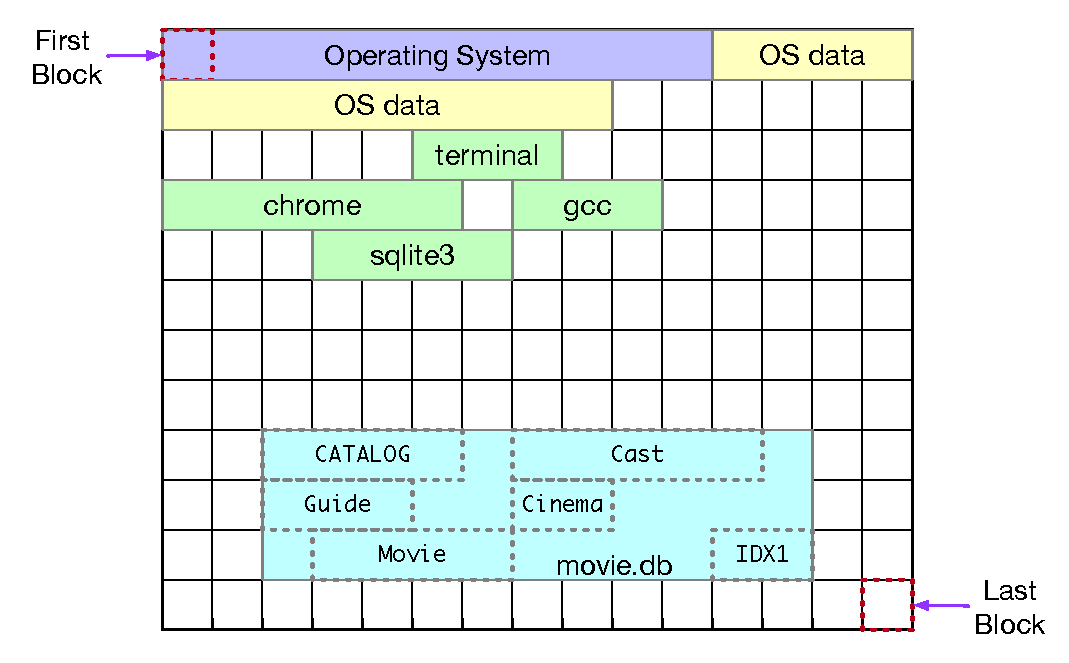
\includegraphics[trim={3.65cm 0.65cm 3.45cm 6.5cm},clip,width=0.6\textwidth]{../lec03_hardware/figures/blocks_on_storage}
\end{center}


Many DBMSs will grab many storage blocks from the Operating System (and leave them empty), to make sure there will be space for growth over time.
\end{frame}


%
% ---------------------------------------------------------------------------
%
\begin{frame}{The database catalog}


The catalog contains the \emph{schemata} of all tables, the description of all indexes and triggers. On multiuser systems, it also contains all users and their privileges.\footnote{Check out the \lstinline[style=cmput391]{-:.schema:-} and \lstinline[style=cmput391]{-:.dump:-} commands in SQLite.}

\vskip1em

The catalog is used all the time: to parse SQL queries, to validate updates, etc. 

Often the DBMS will bring the entire catalog to memory as part of the startup process.

\vskip1em

In most systems, the catalog is actually represented as a collection of tables, which the database administrator can inspect using SQL queries.

\vskip1em

\end{frame}


%
% ---------------------------------------------------------------------------
%
\begin{frame}{Heap files}

The most common kind of DBMS file, called a heap file, is just a \underline{chain of blocks}, with each block containing several \textbf{records}.

Each record represents a database object (e.g., a whole tuple).

\vskip2em

\begin{center}
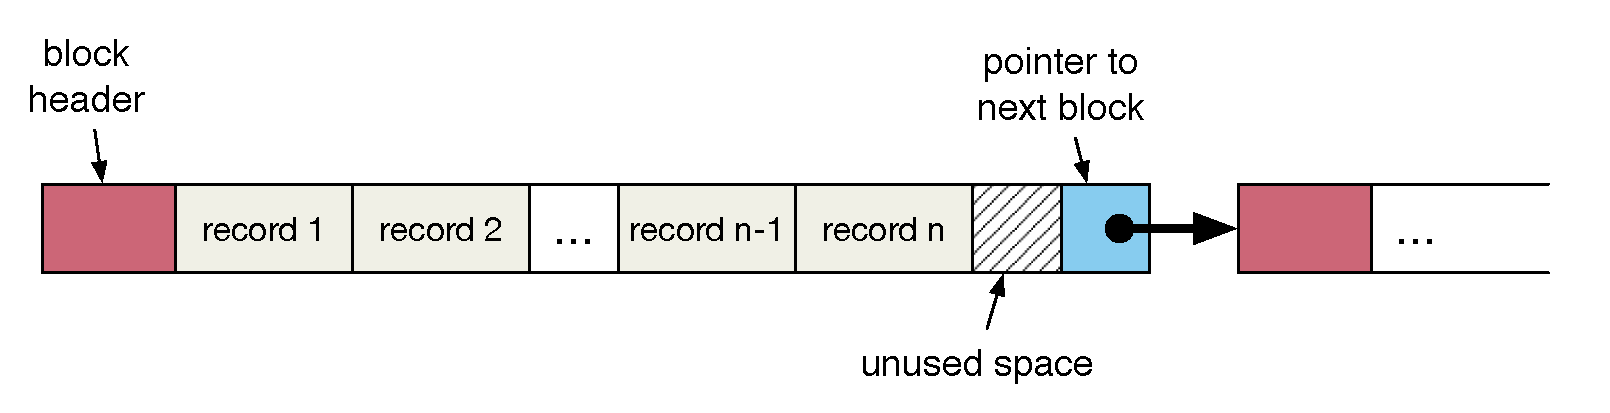
\includegraphics[width=0.9\textwidth]{figures/heap_file}
\end{center}

\end{frame}


%
% ---------------------------------------------------------------------------
%
\begin{frame}

Records have a header (metadata) and a payload (data):

\begin{center}
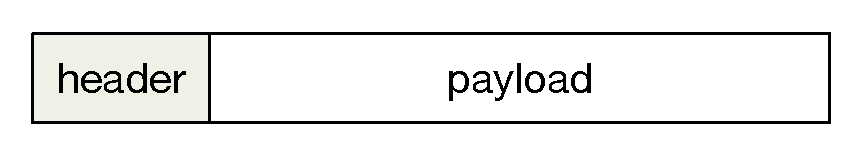
\includegraphics[width=0.5\textwidth]{figures/generic_record}
\end{center}

In a \emph{tuple-oriented store}, each record in a ``table file'' corresponds to a whole tuple\footnote{Except for \lstinline[style=cmput391]{BLOB} (Binary Large OBjects) values like images, sound, etc., in which the record has a pointer to the actual \lstinline[style=cmput391]{BLOB} object.}.

In this case, the header typically contains:
\begin{itemize}[-,noitemsep,topsep=-0.5em]
\item A pointer to the catalog--where the data types of the attributes in the tuple are described.
\item A timestamp of the last update.
\item A flag indicating if the record is valid (or has been deleted).\footnote{It is much cheaper to implement deletions by just marking tuples this way.}
\end{itemize}

\vskip1em
~
\end{frame}


%
% ---------------------------------------------------------------------------
%
\begin{frame}
\label{tuple_oriented_stores}

If the lengths of all attributes in a tuple are defined in the schema, the DBMS can use \textbf{fixed-length records}.

\begin{itemize}[-]
\item In this scheme, every field of the record lies at a constant \emph{offset} from the address where the record is loaded in memory.
\end{itemize}
 

\vskip 0.5em
Example:
\vskip 0.5em

%%% create table stament
\fbox{\usebox{\SimplifiedMovieTableDDL}}

\vskip 0.5em

The record would look like:
\begin{center}
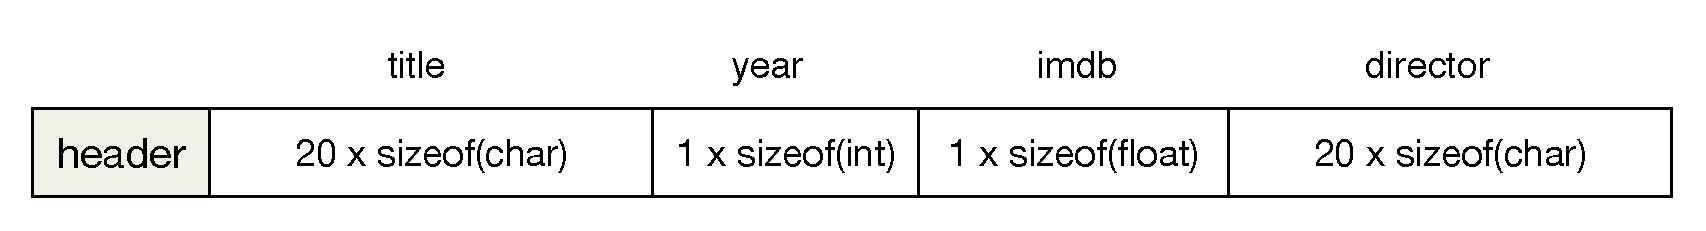
\includegraphics[width=0.95\textwidth]{figures/fixed_record_movie}
\end{center}
\end{frame}


%
% ---------------------------------------------------------------------------
%
\begin{frame}

Fixed-length records can be wasteful for \lstinline[style=SQL]{NULL} values and textual attributes (e.g., names, addresses, etc.) because of variability in the length of actual values.\footnote{SQL has data types for varying-length textual data like \texttt{VARCHAR} and \texttt{TEXT}.}

With \textbf{variable-length} records, instead of ``padding blanks'' special codes as acting as \emph{field delimiters} are used.

\begin{figure}
\begin{subfigure}{0.22\textwidth}
\hfill Fixed
\end{subfigure}
~
\begin{subfigure}{0.74\textwidth}
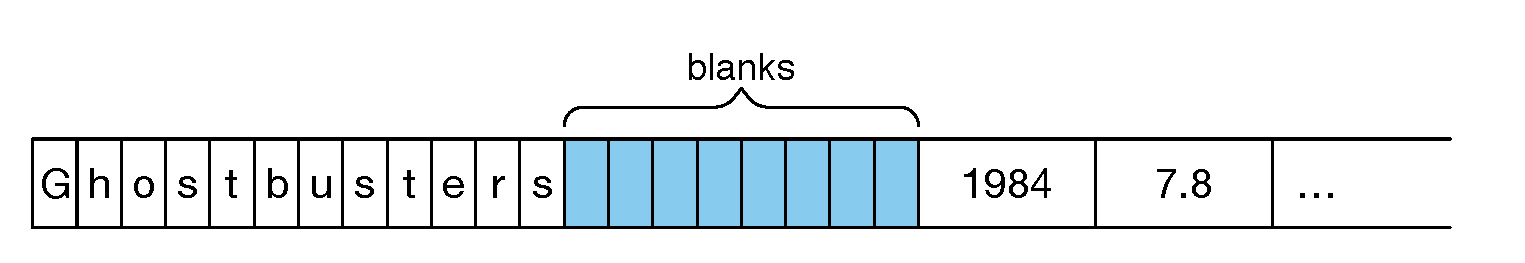
\includegraphics[width=\textwidth]{figures/fixed_length_example}
\end{subfigure}
\end{figure}

\begin{figure}
\begin{subfigure}{0.22\textwidth}
\hfill Variable
\end{subfigure}
~
\begin{subfigure}{0.74\textwidth}
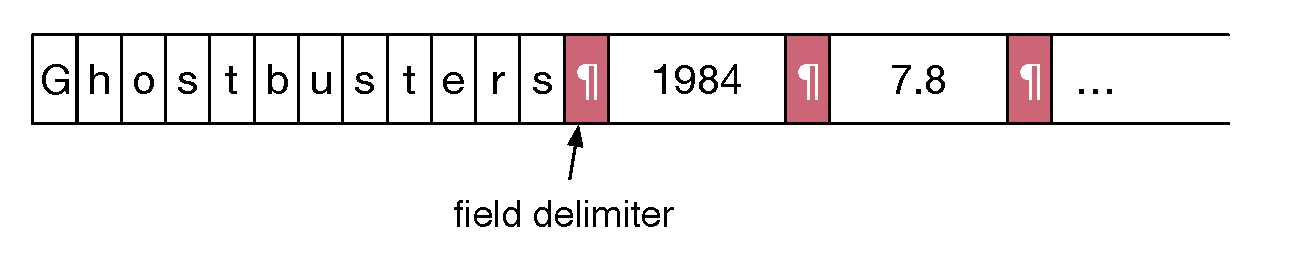
\includegraphics[width=0.85\textwidth]{figures/variable_length_example}
\end{subfigure}
\end{figure}
\end{frame}

%
% ---------------------------------------------------------------------------
%
\begin{frame}

If \lstinline[style=cmput391]{NULL} values are common in the data it is best to use both field delimiters \emph{and} \textbf{field codes}; in this way the record contains only the fields whose values are not missing:

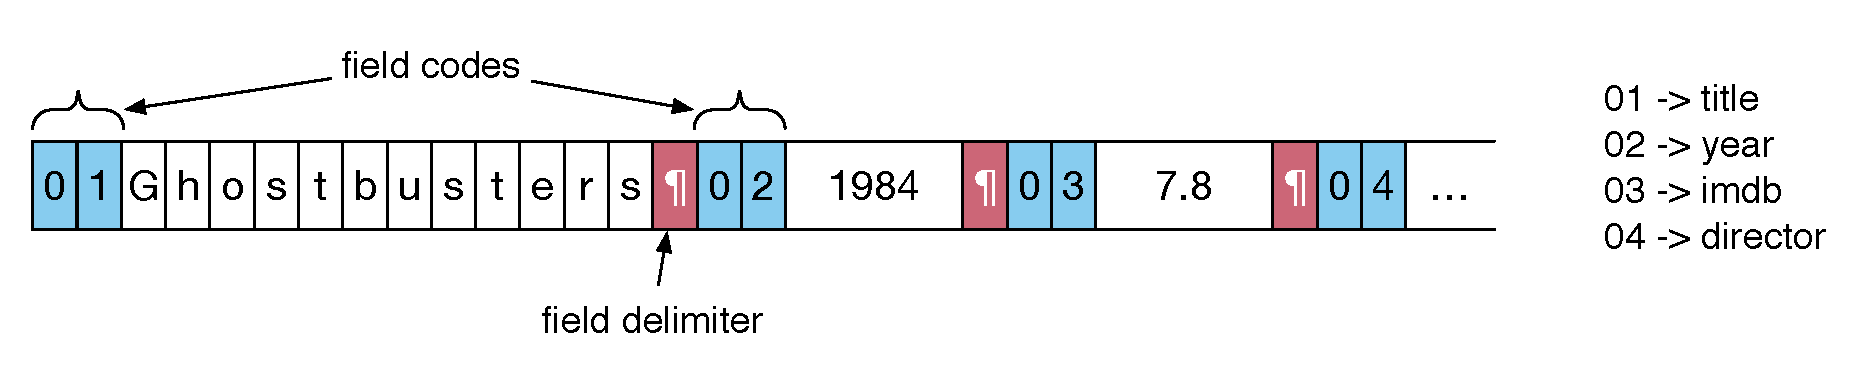
\includegraphics[width=\textwidth]{figures/variable_length_field_codes.eps}

\vskip1em

This kind of record can be used for non-relational data too, like semi-structured or XML.

\end{frame}

%
% ---------------------------------------------------------------------------
%
\begin{frame}{Packing records into buffers/blocks}
\label{heap_file}
Regardless of the kind of record, most stores pack as many whole records into a block as possible. Space that is smaller than a record is \emph{left unused}.

\vskip1em

\begin{center}
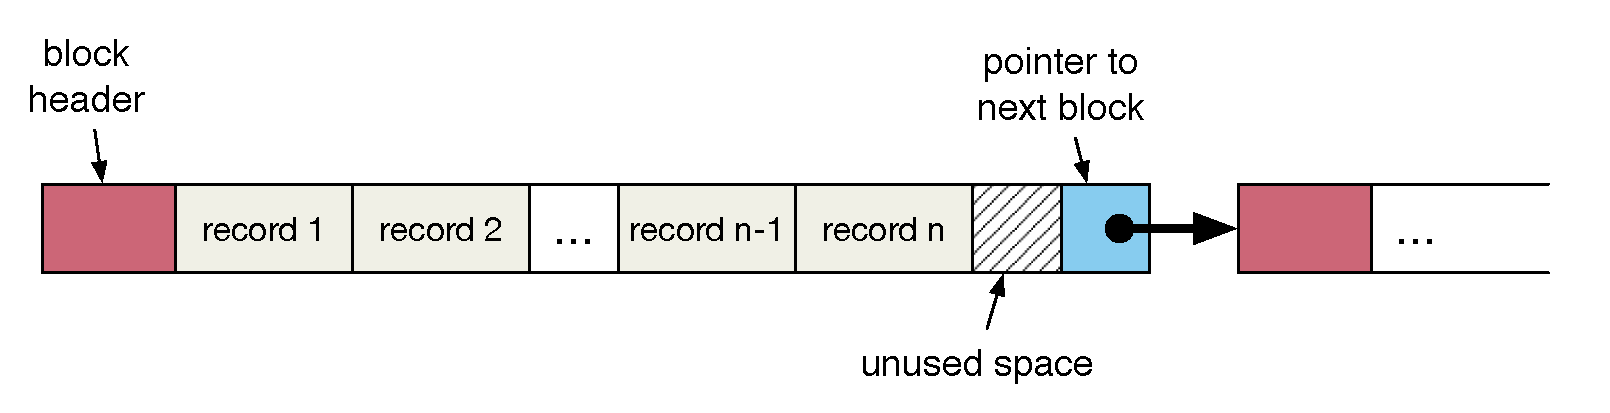
\includegraphics[width=0.9\textwidth]{figures/heap_file}
\end{center}

It is possible to allow a record to \emph{span} consecutive blocks, but the trouble is often not worth it.

\end{frame}


%
% ---------------------------------------------------------------------------
%
\begin{frame}

\textbf{Fixed-length records}:
\begin{itemize}[-,topsep=-0.5em]
\item Fixed number of records per block: \(\floor*{\frac{\text{block size}}{\text{record size}}}\) .

\item Space wasted on ``blanks''.

\item Records and fields start at known \emph{offsets} within the block.
\end{itemize}

\vfill

\textbf{Variable-length records}:

\begin{itemize}[-,topsep=-0.5em]
\item Variable number of records per block.

\item Space ``wasted'' on field separators.

\item Need to scan the whole block to find records and fields.

\item Can be used to store non-relational, semi-structured data.
\end{itemize}

\end{frame}


%
% ---------------------------------------------------------------------------
%
\begin{frame}{ASIDE: word-aligned data structures}
Once a record is loaded in memory, a processor in the CPU can get to a field by manipulating offsets or scanning through the record.

However, some CPUs allow reading/writing entire \textbf{words}\footnote{\url{https://en.wikipedia.org/wiki/Data_structure_alignment}} (4 or 8 bytes, depending on the architecture) only.

When this happens, either the storage stack aligns the fields, which is wasteful,\footnote{Some CPUs, on the other hand, allow access to individual bytes inside each word.} or it contains code to properly ``encode'' and ``decode'' fields into words.
\end{frame}

%
% ---------------------------------------------------------------------------
%
\begin{frame}

Example record:\\
- \texttt{f1}: 5 UTF-16 (2 bytes) characters\\
- \texttt{f2}: 1 Boolean value (1 bit)\\
- \texttt{f3}: 1 \texttt{smallint} (2 bytes)

\begin{figure}
\begin{subfigure}{0.25\textwidth}
\hfill Un-aligned 
\end{subfigure}
~~
\begin{subfigure}{0.7\textwidth}
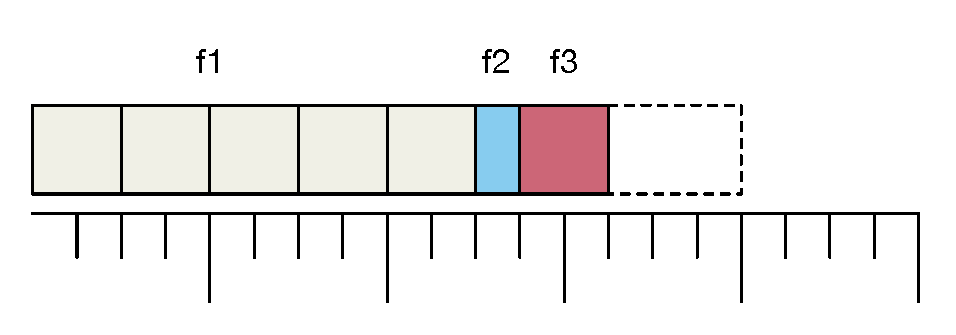
\includegraphics[width=0.8\textwidth]{figures/record_unaligned}
\end{subfigure}
\end{figure}

\begin{figure}
\begin{subfigure}{0.25\textwidth}
\hfill Aligned 
\end{subfigure}
~~
\begin{subfigure}{0.7\textwidth}
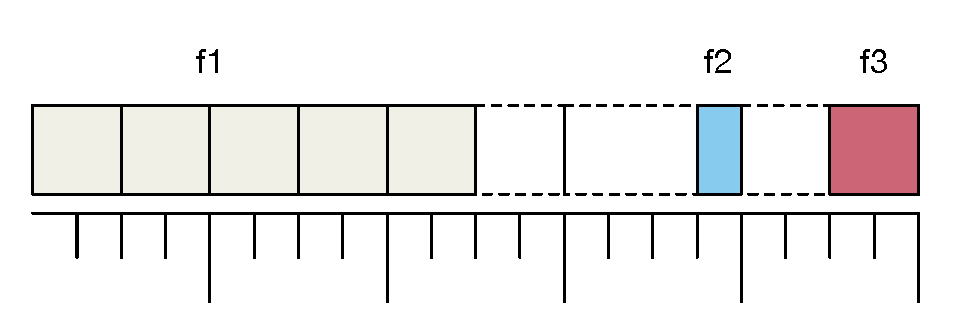
\includegraphics[width=0.8\textwidth]{figures/record_aligned}
\end{subfigure}
\end{figure}

\end{frame}


